\section{Game engine architecture}
The game engine forms an environment for the agent by keeping track of the game state (including scores), providing the available actions (moves), and generating possible future states and their probabilities in the game tree based on the current knowledge.
The number of possible states in Carcassonne quickly rises as more tiles are placed on the board leading to its high branching factor ($b = 55$ on average \cite{MasterThesisCarcassonne}).
To maximize the number of states that can be included in the search tree, the team opted to implement the game engine from scratch using a fast compilable language to later bridge it with an agent implemented in a language that is better suited for developing AI applications.

This section will focus on the architecture of this engine and how the communication within the whole system works.

\subsection{Overview of architecture}
% Opisanie architektury silnika, sposobu komunikacji między komponentami, a także za co one odpowiadają.

In this section, the project of game architecture will be discussed.
\ref{fig:SystemArchitecture} shows a diagram of the whole system as implemented by the team.
Computations related to processing games are performed on a CPU,
while agents should be trained on a GPU.

\begin{figure*}
	\centering
	\scalebox{.48}{% Generated with:
% $ java -jar plantuml.jar -tlatex:nopreamble arch.pu
% generated by Plantuml 1.2024.8
\definecolor{plantucolor0000}{RGB}{24,24,24}
\definecolor{plantucolor0001}{RGB}{0,0,0}
\definecolor{plantucolor0002}{RGB}{241,241,241}
\begin{tikzpicture}[yscale=-1
,pstyle0/.style={color=plantucolor0000,line width=1.0pt}
,pstyle1/.style={color=black,line width=1.5pt}
,pstyle2/.style={color=plantucolor0000,fill=plantucolor0002,line width=0.5pt}
,pstyle3/.style={color=plantucolor0000,line width=0.5pt}
,pstyle5/.style={color=plantucolor0000,fill=plantucolor0000,line width=1.0pt}
,pstyle6/.style={color=plantucolor0000,line width=4.0pt}
,pstyle7/.style={color=plantucolor0000,fill=plantucolor0000,line width=4.0pt}
]
\draw[pstyle0] (38pt,97pt) -- (48pt,87pt) -- (517pt,87pt) -- (517pt,352pt) -- (507pt,362pt) -- (38pt,362pt) -- (38pt,97pt) -- cycle;
\draw[pstyle0] (507pt,97pt) -- (517pt,87pt);
\draw[pstyle0] (38pt,97pt) -- (507pt,97pt);
\draw[pstyle0] (507pt,97pt) -- (507pt,362pt);
\node at (260.99pt,100pt)[below right,color=black,inner sep=0]{\textbf{CPU}};
\draw[pstyle1] (196.5pt,129pt) -- (261.53pt,129pt) arc(270:360:3.75pt)  -- (271.03pt,145pt) -- (456.5pt,145pt) arc(270:360:2.5pt)  -- (459pt,335.5pt) arc(0:90:2.5pt)  -- (196.5pt,338pt) arc(90:180:2.5pt)  -- (194pt,131.5pt) arc(180:270:2.5pt) ;
\draw[pstyle1] (194pt,145pt) -- (271.03pt,145pt);
\node at (198pt,131pt)[below right,color=black,inner sep=0]{\textbf{GameEngine}};
\draw[pstyle0] (16pt,416pt) -- (26pt,406pt) -- (158pt,406pt) -- (158pt,486pt) -- (148pt,496pt) -- (16pt,496pt) -- (16pt,416pt) -- cycle;
\draw[pstyle0] (148pt,416pt) -- (158pt,406pt);
\draw[pstyle0] (16pt,416pt) -- (148pt,416pt);
\draw[pstyle0] (148pt,416pt) -- (148pt,496pt);
\node at (70.125pt,419pt)[below right,color=black,inner sep=0]{\textbf{GPU}};
\draw[pstyle2] (94.5pt,148pt) arc (180:270:5pt) -- (99.5pt,143pt) -- (172.14pt,143pt) arc (270:360:5pt) -- (177.14pt,148pt) -- (177.14pt,178pt) arc (0:90:5pt) -- (172.14pt,183pt) -- (99.5pt,183pt) arc (90:180:5pt) -- (94.5pt,178pt) -- cycle;
\draw[pstyle2] (157.14pt,148pt) rectangle (172.14pt,158pt);
\draw[pstyle2] (155.14pt,150pt) rectangle (159.14pt,152pt);
\draw[pstyle2] (155.14pt,154pt) rectangle (159.14pt,156pt);
\node at (109.5pt,163pt)[below right,color=black,inner sep=0]{Visualiser};
\draw[pstyle2] (54.5pt,284pt) arc (180:270:5pt) -- (59.5pt,279pt) -- (172.73pt,279pt) arc (270:360:5pt) -- (177.73pt,284pt) -- (177.73pt,314pt) arc (0:90:5pt) -- (172.73pt,319pt) -- (59.5pt,319pt) arc (90:180:5pt) -- (54.5pt,314pt) -- cycle;
\draw[pstyle2] (157.73pt,284pt) rectangle (172.73pt,294pt);
\draw[pstyle2] (155.73pt,286pt) rectangle (159.73pt,288pt);
\draw[pstyle2] (155.73pt,290pt) rectangle (159.73pt,292pt);
\node at (69.5pt,299pt)[below right,color=black,inner sep=0]{TrainingSupervisor};
\draw[pstyle2] (338.5pt,153pt) -- (401.02pt,153pt) ..controls (406.02pt,153pt) and (406.02pt,163pt) .. (406.02pt,163pt) ..controls (406.02pt,163pt) and (406.02pt,173pt) .. (401.02pt,173pt) -- (338.5pt,173pt) ..controls (333.5pt,173pt) and (333.5pt,163pt) .. (333.5pt,163pt) ..controls (333.5pt,163pt) and (333.5pt,153pt) .. (338.5pt,153pt);
\draw[pstyle3] (401.02pt,153pt) ..controls (396.02pt,153pt) and (396.02pt,163pt) .. (396.02pt,163pt) ..controls (396.02pt,173pt) and (401.02pt,173pt) .. (401.02pt,173pt);
\node at (338.5pt,158pt)[below right,color=black,inner sep=0]{BatchBuffer};
\draw[pstyle2] (253.5pt,289pt) arc (180:270:5pt) -- (258.5pt,284pt) -- (305.23pt,284pt) arc (270:360:5pt) -- (310.23pt,289pt) -- (310.23pt,309pt) arc (0:90:5pt) -- (305.23pt,314pt) -- (258.5pt,314pt) arc (90:180:5pt) -- (253.5pt,309pt) -- cycle;
\node at (263.5pt,294pt)[below right,color=black,inner sep=0]{Worker1};
\draw[pstyle2] (345.5pt,289pt) arc (180:270:5pt) -- (350.5pt,284pt) -- (397.23pt,284pt) arc (270:360:5pt) -- (402.23pt,289pt) -- (402.23pt,309pt) arc (0:90:5pt) -- (397.23pt,314pt) -- (350.5pt,314pt) arc (90:180:5pt) -- (345.5pt,309pt) -- cycle;
\node at (355.5pt,294pt)[below right,color=black,inner sep=0]{Worker2};
\node at (428.075pt,203pt)[below right,color=black,inner sep=0]{LoggerOutput};
\draw[color=plantucolor0000,fill=plantucolor0002,line width=1.5pt] (453pt,225pt) rectangle (465pt,237pt);
\draw[pstyle2] (32.5pt,445pt) arc (180:270:5pt) -- (37.5pt,440pt) -- (136.7pt,440pt) arc (270:360:5pt) -- (141.7pt,445pt) -- (141.7pt,475pt) arc (0:90:5pt) -- (136.7pt,480pt) -- (37.5pt,480pt) arc (90:180:5pt) -- (32.5pt,475pt) -- cycle;
\draw[pstyle2] (121.7pt,445pt) rectangle (136.7pt,455pt);
\draw[pstyle2] (119.7pt,447pt) rectangle (123.7pt,449pt);
\draw[pstyle2] (119.7pt,451pt) rectangle (123.7pt,453pt);
\node at (47.5pt,460pt)[below right,color=black,inner sep=0]{Pytorch/CUDA};
\draw[pstyle2] (263.5pt,12pt) arc (180:270:5pt) -- (268.5pt,7pt) -- (327.52pt,7pt) arc (270:360:5pt) -- (332.52pt,12pt) -- (332.52pt,35pt) arc (0:90:5pt) -- (327.52pt,40pt) -- (268.5pt,40pt) arc (90:180:5pt) -- (263.5pt,35pt) -- cycle;
\draw[pstyle2] (315.52pt,12pt) -- (315.52pt,26pt) -- (327.52pt,26pt) -- (327.52pt,18pt) -- (321.52pt,12pt) -- (315.52pt,12pt) -- cycle;
\draw[pstyle3] (321.52pt,12pt) -- (321.52pt,18pt);
\draw[pstyle3] (327.52pt,18pt) -- (321.52pt,18pt);
\node at (273.5pt,20pt)[below right,color=black,inner sep=0]{gameLog};
\draw[pstyle0] (363.95pt,173.21pt) ..controls (348.88pt,196.15pt) and (312.8842pt,250.9752pt) .. (294.7342pt,278.6052pt);
\draw[pstyle5] (291.44pt,283.62pt) -- (299.7245pt,278.2939pt) -- (294.1852pt,279.441pt) -- (293.0381pt,273.9017pt) -- (291.44pt,283.62pt) -- cycle;
\draw[pstyle0] (370.27pt,173.21pt) ..controls (370.96pt,196.15pt) and (372.572pt,249.9926pt) .. (373.392pt,277.6226pt);
\draw[pstyle5] (373.57pt,283.62pt) -- (377.3013pt,274.5053pt) -- (373.4217pt,278.6222pt) -- (369.3048pt,274.7426pt) -- (373.57pt,283.62pt) -- cycle;
\draw[pstyle0] (338.3696pt,32.1399pt) ..controls (366.7796pt,39.0599pt) and (400.13pt,51.68pt) .. (423pt,79pt) ..controls (461.23pt,124.67pt) and (460.28pt,204.02pt) .. (459.31pt,224.87pt);
\draw[pstyle5] (332.54pt,30.72pt) -- (340.3377pt,36.7363pt) -- (337.398pt,31.9033pt) -- (342.231pt,28.9635pt) -- (332.54pt,30.72pt) -- cycle;
\draw[pstyle0] (263.53pt,40.02pt) ..controls (244.27pt,49.64pt) and (220.5pt,63.18pt) .. (202pt,79pt) ..controls (180.04pt,97.79pt) and (160.19pt,124.75pt) .. (148.12pt,142.79pt);
\draw[pstyle6] (188.2564pt,194.6698pt) ..controls (169.7577pt,203.2148pt) and (157.425pt,209.51pt) .. (154pt,213pt) ..controls (135.89pt,231.47pt) and (125.58pt,260.05pt) .. (120.39pt,278.9pt);
\draw[pstyle7] (193.7074pt,192.1624pt) -- (183.8594pt,192.2895pt) -- (189.1649pt,194.2519pt) -- (187.2025pt,199.5575pt) -- (193.7074pt,192.1624pt) -- cycle;
\node at (155pt,226pt)[below right,color=black,inner sep=0]{Action};
\draw[pstyle6] (193.7154pt,243.6133pt) ..controls (193.6039pt,243.7216pt) and (193.4923pt,243.8298pt) .. (193.3808pt,243.9378pt) ..controls (191.5955pt,245.6666pt) and (189.8006pt,247.3569pt) .. (188pt,249pt) ..controls (175.94pt,260.01pt) and (166.2778pt,267.1911pt) .. (153.3078pt,275.5811pt);
\draw[pstyle7] (148.27pt,278.84pt) -- (157.9993pt,277.3103pt) -- (152.4682pt,276.1243pt) -- (153.6542pt,270.5931pt) -- (148.27pt,278.84pt) -- cycle;
\node at (221pt,226pt)[below right,color=black,inner sep=0]{NewGameState};
\draw[pstyle6] (90.47pt,319.04pt) ..controls (73.75pt,333.2pt) and (53.33pt,354.14pt) .. (44pt,378pt) ..controls (35.36pt,400.09pt) and (47.2722pt,419.5087pt) .. (62.1422pt,435.5587pt);
\draw[pstyle7] (66.22pt,439.96pt) -- (63.0376pt,430.6395pt) -- (62.8219pt,436.2922pt) -- (57.1691pt,436.0765pt) -- (66.22pt,439.96pt) -- cycle;
\node at (45pt,379pt)[below right,color=black,inner sep=0]{NewGameState};
\draw[pstyle6] (119.1934pt,325.1575pt) ..controls (121.1134pt,343.5375pt) and (122pt,365.98pt) .. (117pt,390pt) ..controls (113.33pt,407.65pt) and (104.9pt,426.32pt) .. (97.91pt,439.78pt);
\draw[pstyle7] (118.57pt,319.19pt) -- (115.5267pt,328.5569pt) -- (119.0895pt,324.1629pt) -- (123.4834pt,327.7257pt) -- (118.57pt,319.19pt) -- cycle;
\node at (120pt,379pt)[below right,color=black,inner sep=0]{Action};
\end{tikzpicture}
}
	\caption{Diagram of the system's architecture}
	\label{fig:SystemArchitecture}
\end{figure*}

The GameEngine is responsible for evaluating requests it receives from the agents
ensuring that the Carcassonne's rule set is followed. It maintains currently active games,
exposes the current state to the agents, generates possible moves for the given input,
and allows to simulate what game state a sequence of actions will lead to (before performing it
on an active game). Internally, GameEngine distributes the requests it receives among
multiple workers (lightweight threads) that can evaluate them simultaneously. Actions that
require state transitions are performed on a state's clone, while read-only operations
get performed on the original copy which is meant to enable efficient concurrency.

For each active game, GameEngine logs all of its states to that game's log file,
allowing for later consumption by Visualiser. Visualiser parses the logs
and presents the game in a graphical form, allowing for analysis by humans.

TrainingSupervisor is responsible for managing communication and supervising agents' training.
It should optimize communication by reducing data transfer between CPU and GPU.

The GameEngine (and Visualiser) is implemented in Go, while the agent and TrainingSupervisor
are implemented in Python. The use of Go for the engine was meant to allow for better performance of
the rule engine but it means that the TrainingSupervisor cannot communicate with it directly.
To solve this, the team used the gopy project \cite{gopy} to automatically generate
Python bindings \cite{LanguageBindings} for the Go package. This leads to a larger overhead than
using manually-written CPython extension would but this has been considered acceptable as most of
CPU-bound work happens in the GameEngine.

\subsection{Components of a solution}
% Opisanie elementów z jakich się składa rozgrywka m.in.: kafelki i ich elementy, gracze, a także uwzględnione rozszerzenia gry Carcassonne.

The game Carcassone is played by placing tiles \cite{CarcassoneRules}. Each tile is represented by a set of features on it. All features are defined by their type, such as road, city, field or monastery, a modifier that modifies the calculation process, and the sides which indicate on which edges the feature is present. In this project there is only one modifier used - the shield. The engine was designed to accommodate game extensions. 

A feature's side is a byte sized value, in which each bit defines whether the feature is present on a specific half of the tile's edge as shown on Figure \ref{fig:SIDES}. Features such as roads, are represented by a whole edge formed by combining two sides e.g., the TopLeft and TopRight sides.
\begin{figure}
    \centering
    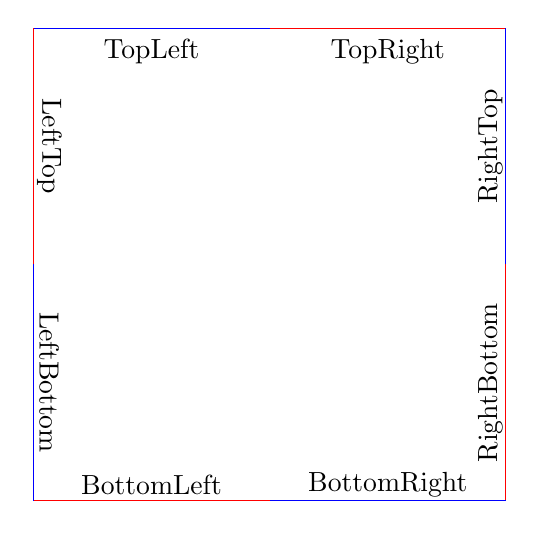
\begin{tikzpicture}
        %top line
        \draw [blue] (-3,3) -- (0,3);
        \draw [red] (0,3) -- (3,3);
        %right line
        \draw [blue] (3,3) -- (3,0);
        \draw [red] (3,0) -- (3,-3);
        %bottom line
        \draw [blue] (3,-3) -- (0,-3);
        \draw [red] (0,-3) -- (-3,-3);
        %left line
        \draw [blue] (-3,-3) -- (-3,0);
        \draw [red] (-3,0) -- (-3,3);
        
        \node at (-1.5, 2.7) {TopLeft};
        \node at (1.5, 2.7) {TopRight};
        
        \node [rotate=90] at (2.8, 1.5) {RightTop};
        \node [rotate=90] at (2.8, -1.5) {RightBottom};
        
        \node at (-1.5, -2.8) {BottomLeft};
        \node at (1.5, -2.8) {BottomRight};
        
	% czy może obrót 90stopni?
        \node [rotate=270] at (-2.8, 1.5) {LeftTop};
        \node [rotate=270] at (-2.8, -1.5) {LeftBottom};
    \end{tikzpicture}
    \caption{Side representation} \label{fig:SIDES}
\end{figure}

The tiles described do not contain information about their position or meeple placement. This information is located in the PlacedTile struct. The board is represented as a tile set containing tiles used in the game, for verification whether the tile a player wants to place is legal,  moreover it contains slice of placed tiles in the same order as a tile set. Additionally, board includes a city manager used for merging cities, scoring and checking for legal meeples placement in the cities.

A single game is represented by a board, shuffled deck of tiles, and players partaking in it. Each player knows their score, and the number of meeples of each type available to them.

Our solution has been designed to be modifiable by adding extensions to the game. Generalizations, such as meeple type or feature type, allow for the easy implementation of new potential features e.g., rivers.

\subsection{Execution flow}
% Opisanie wykonywanych akcji podejmowanych przez silnik gry: wylosowanie kafelka ze stosu, wyliczenie legalnych ułożeń kafelka, wybór położenia i wyliczanie punktacji za jego położenie.
Lorem ipsum dolor sit amet, consectetur adipiscing elit. Nam consectetur dignissim urna, a rhoncus dolor venenatis adipiscing. Phasellus viverra aliquam fringilla. Praesent mattis diam id ipsum placerat a laoreet diam tempus. Quisque eu leo ut sapien ultricies gravida ac sed turpis. Donec nibh enim, pretium a sagittis et, varius non nulla. Vivamus enim augue, condimentum eget convallis hendrerit, mattis ut lectus. Cum sociis natoque penatibus et magnis dis parturient montes, nascetur ridiculus mus. Proin semper libero augue. Praesent auctor ligula sit amet quam molestie adipiscing. Mauris vehicula congue mollis. Duis tincidunt interdum purus quis congue. Integer vel orci mauris. Curabitur rutrum tincidunt mi ut elementum. Nunc non massa nunc. Donec ultricies ipsum ac risus sollicitudin porta. Phasellus elementum odio et leo consectetur consectetur. 

Lorem ipsum dolor sit amet, consectetur adipiscing elit. Nam consectetur dignissim urna, a rhoncus dolor venenatis adipiscing. Phasellus viverra aliquam fringilla. Praesent mattis diam id ipsum placerat a laoreet diam tempus. Quisque eu leo ut sapien ultricies gravida ac sed turpis. Donec nibh enim, pretium a sagittis et, varius non nulla. Vivamus enim augue, condimentum eget convallis hendrerit, mattis ut lectus. Cum sociis natoque penatibus et magnis dis parturient montes, nascetur ridiculus mus. Proin semper libero augue. Praesent auctor ligula sit amet quam molestie adipiscing. Mauris vehicula congue mollis. Duis tincidunt interdum purus quis congue. Integer vel orci mauris. Curabitur rutrum tincidunt mi ut elementum. Nunc non massa nunc. Donec ultricies ipsum ac risus sollicitudin porta. Phasellus elementum odio et leo consectetur consectetur. 

\subsection{Communication within a system}
% Opisanie komunikacji pomiędzy silnikiem gry, a sieciami neuronowymi uczonymi na karcie graficznej. Aktualizacja stanu gry w zależności od akcji podejmowanych przez agenta.

The game engine is capable of handling multiple game instances, by using Go pipelines and goroutines \cite{GolangPipeline}, which allows for many agents to play and learn simultaneously. The engine provides several request types necessary for the agents, to retrieve information about the game. There are five such requests:
\begin{itemize}
    \item CloneGame - used for creating a separate clone of a game. It allows the agent to expand the game tree, and each clone can be modified by the agent, by simulating its next potential move.
    \item GetRemainingTiles - returns all available tiles that have not yet been placed. With this data, the agent can expand the game tree for each possible move that might occur. The returned tiles come with information about their probability.
    \item GetLegalMoves - returns all legal moves for a given tile. It considers where the tile can be placed and where are the possible meeple placements on it.
    \item GetMidGameScore - returns the information about the score for all players, calculated as if the game has just finished.
    \item PlayTurn - allows the agent to play a turn using a given tile, and modifies the game state. It returns the new state of the game 
\end{itemize}

% coś o tym że  agent może budować drzewo jak w algorytmie alphago, ale troche nie wiem jak ten akapit rozwinąć.
With these requests, the agent is capable of building its own game tree, as in the AlphaGo algorithm \cite{AlphaGoAlgorithm}.

To provide the neural network with the game state, a serialization process is required. Serialized game contains all players' statistics (meeple counts, score) and all tiles on the board. The placed tiles on the board are represented in the binary format to ensure a fixed memory size of 8 bytes. The slice of binary tiles consists of all tiles in the same order as tiles in tile set. The tiles in this array that are not yet placed are set to zero.
